% Created 2019-08-19 lun. 13:52
% Intended LaTeX compiler: pdflatex
\documentclass[letterpaper, 10 pt, conference]{ieeeconf}
\usepackage[utf8]{inputenc}
\usepackage[T1]{fontenc}
\usepackage{graphicx}
\usepackage{grffile}
\usepackage{longtable}
\usepackage{wrapfig}
\usepackage{rotating}
\usepackage[normalem]{ulem}
\usepackage{amsmath}
\usepackage{textcomp}
\usepackage{amssymb}
\usepackage{capt-of}
\usepackage{hyperref}
\usepackage[most]{tcolorbox}
\usepackage{siunitx}
\usepackage{amsmath,amssymb,amsfonts, cases}
\usepackage[noadjust,space,compress]{cite}
\usepackage{tabularx,siunitx,booktabs}
\usepackage{algorithmic, graphicx, textcomp}
\usepackage{xcolor, import, hyperref}
\usepackage[USenglish, english]{babel}
\setcounter{footnote}{1}
\renewcommand{\citedash}{--}
\IEEEoverridecommandlockouts
\author{Dehaeze Thomas\textsuperscript{1,2,$\dagger$}, Verma Mohit\textsuperscript{1,3} and Collette Christophe\textsuperscript{1,3}  \thanks{\textsuperscript{1} Precision Mechatronics Laboratory, A\&M Department, Liege, Belgium} \thanks{\textsuperscript{2} European Synchrotron Radiation Facility, Grenoble, France} \thanks{\textsuperscript{3} Unversité Libre de Bruxelles, BEAMS Department, Brussels, Belgium} \thanks{\textsuperscript{$\dagger$} Email: {\tt\small thomas.dehaeze@esrf.fr}}}
\date{2019-08-19}
\title{Design of Complementary Filters Using the \(\mathcal{H}_\infty\) Synthesis}
\hypersetup{
 pdfauthor={Dehaeze Thomas\textsuperscript{1,2,$\dagger$}, Verma Mohit\textsuperscript{1,3} and Collette Christophe\textsuperscript{1,3}  \thanks{\textsuperscript{1} Precision Mechatronics Laboratory, A\&M Department, Liege, Belgium} \thanks{\textsuperscript{2} European Synchrotron Radiation Facility, Grenoble, France} \thanks{\textsuperscript{3} Unversité Libre de Bruxelles, BEAMS Department, Brussels, Belgium} \thanks{\textsuperscript{$\dagger$} Email: {\tt\small thomas.dehaeze@esrf.fr}}},
 pdftitle={Design of Complementary Filters Using the \(\mathcal{H}_\infty\) Synthesis},
 pdfkeywords={},
 pdfsubject={},
 pdfcreator={Emacs 26.2 (Org mode 9.2.5)},
 pdflang={English}}
\begin{document}

\maketitle
\bibliographystyle{IEEEtran}

\begin{abstract}
Abstract text to be done
\end{abstract}

\section{Introduction}
\label{sec:org1868519}
\label{sec:introduction}
A set of filters is said to be complementary if the sum of their transfer functions is equal to one at all frequencies.
These filters are used when two or more sensors are measuring the same physical quantity with different noise characteristics. Unreliable frequencies of each sensors are filtered out by the complementary filters and combined to form a "super sensor" giving a better estimate of the physical quantity over a wider bandwidth.
This technique is called sensor blending or sensor fusion and used for many applications.\par
In \cite{zimmermann92_high_bandw_orien_measur_contr,corke04_inert_visual_sensin_system_small_auton_helic,min15_compl_filter_desig_angle_estim}, such technique is used for the attitude estimation of Unmanned Aerial Vehicles (UAV) using various sensors (accelerometers, gyroscopes, vision sensors, \ldots{}).
In \cite{collette15_sensor_fusion_method_high_perfor}, several sensor fusion configurations using different types of sensors (inertial, relative motion and force) have been discussed in order to increase the control bandwidth of active vibration isolation systems.
Furthermore, sensor fusion is used for the low frequency isolation at the Laser Interferometer Gravitational-Wave Observator (LIGO), where inertial sensors are merged with relative sensors
\cite{matichard15_seism_isolat_advan_ligo,hua04_polyp_fir_compl_filter_contr_system}. \par
As the super sensor noise characteristics depends largely on the complementary filter norms, their proper design is of primary importance for sensor fusion performance.
Different design methods have been developed.
In \cite{corke04_inert_visual_sensin_system_small_auton_helic,jensen13_basic_uas,min15_compl_filter_desig_angle_estim}, analytical formulas for complementary filter transfer functions of first and second order have been proposed.
Higher order complementary filters have been used in
\cite{shaw90_bandw_enhan_posit_measur_using_measur_accel,zimmermann92_high_bandw_orien_measur_contr,collette15_sensor_fusion_method_high_perfor}.
In \cite{jensen13_basic_uas}, the sensitivity and complementary sensitivity transfer functions of a feedback architecture have been proposed to be used for complementary filters. The design of such filters can then benefits from the developments of classical control theory.
Linear Matrix Inequalities (LMIs) are used in \cite{pascoal99_navig_system_desig_using_time} for the synthesis of complementary filters satisfying some frequency-like performance.
A design method using linear least squares to optimize the coefficients of complementary filters is proposed in \cite{min15_compl_filter_desig_angle_estim}.
Finally, high order Finite Impulse Response (FIR) complementary filters are used to merge sensors at LIGO \cite{hua05_low_ligo,hua04_polyp_fir_compl_filter_contr_system,matichard15_seism_isolat_advan_ligo}. The synthesis of such filter using convex optimization is presented in \cite{hua05_low_ligo}. \par
Although many design methods of complementary filters have been proposed, we believe that it lacks a simple method of designing complementary filters [\ldots{}] specifying upper bounds.\par
In this paper, we propose a synthesis method for the shaping of complementary filters using the \(\mathcal{H}_\infty\) norm.\par
The section \ref{sec:requirements} gives a brief overview of sensor fusion using complementary filters and the associated requirements on their norms.
In section \ref{sec:hinf_method}, a new method for designing complementary filters using the \(\mathcal{H}_\infty\) synthesis is proposed.
In section \ref{sec:application_ligo}, two high order complementary filters are designed using the proposed method and compared with FIR filters used for sensor fusion at the LIGO.
Our conclusions are drawn in the final section.

\section{Complementary Filters Requirements}
\label{sec:org8f2a1a9}
\label{sec:requirements}
\subsection{Sensor Fusion Architecture}
\label{sec:org202d271}
\label{sec:sensor_fusion}

Let's consider two sensors measuring the same physical quantity \(x\) but with different dynamics (\(G_1(s)\) and \(G_2(s)\)) and noise characteristics (\(n_1\) and \(n_2\)).

The signals from both sensors are fed into two complementary filters \(H_1(s)\) and \(H_2(s)\) and then combined to yield an estimate \(\hat{x}\) of \(x\) as shown on Fig. \ref{fig:fusion_super_sensor}.
\begin{equation}
\label{eq:comp_filter_estimate}
  \hat{x} = \left(G_1 H_1 + G_2 H_2\right) x + H_1 n_1 + H_2 n_2
\end{equation}

\begin{figure}[htbp]
\centering
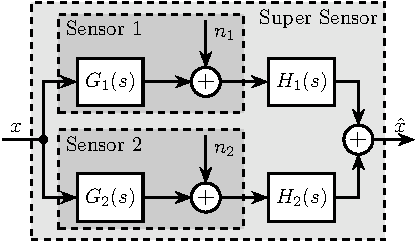
\includegraphics[scale=1]{figs/fusion_super_sensor.pdf}
\caption{\label{fig:fusion_super_sensor}
Sensor Fusion Architecture}
\end{figure}

The complementary property of \(H_1(s)\) and \(H_2(s)\) implies that their transfer function sum is equal to one at all frequencies \eqref{eq:comp_filter}.
\begin{equation}
\label{eq:comp_filter}
  H_1(s) + H_2(s) = 1
\end{equation}

\subsection{Noise Sensor Filtering}
\label{sec:org0ee5b17}
\label{sec:noise_filtering}

Let's first consider sensors with perfect dynamics
\begin{equation}
\label{eq:perfect_dynamics}
  G_1(s) = G_2(s) = 1
\end{equation}

The estimate \(\hat{x}\) is then described by
\begin{equation}
\label{eq:estimate_perfect_dyn}
  \hat{x} = x + H_1 n_1 + H_2 n_2
\end{equation}

The complementary filters \(H_1(s)\) and \(H_2(s)\) only operates on the noise of the sensors.
Thus, this sensor fusion architecture permits to filter the noise of both sensors without introducing any distortion in the physical quantity to measure.

The estimation error \(\delta x\) is defined by \eqref{eq:estimate_error}.
\begin{equation}
\label{eq:estimate_error}
  \delta x \triangleq \hat{x} - x = H_1 n_1 + H_2 n_2
\end{equation}

As shown in \eqref{eq:noise_filtering_psd}, the Power Spectral Density (PSD) of the estimation error \(\Phi_{\delta x}\) depends both on the norms of the complementary filters and on the PSD of the noise sources \(\Phi_{n_1}\) and \(\Phi_{n_2}\).
\begin{equation}
\label{eq:noise_filtering_psd}
  \Phi_{\delta x} = \left|H_1\right|^2 \Phi_{n_1} + \left|H_2\right|^2 \Phi_{n_2}
\end{equation}

Usually, the two sensors have higher noise levels over distinct yet complementary frequency regions.
In order to lower the noise present in the estimation \(\hat{x}\), the norm \(|H_1|\) has to be made small when \(\Phi_{n_1}\) is larger than \(\Phi_{n_2}\) and \(|H_2|\) small when \(\Phi_{n_2}\) is larger than \(\Phi_{n_1}\).


\subsection{Robustness of the Fusion}
\label{sec:orgb942694}
\label{sec:fusion_robustness}

In practical systems, the sensors dynamics has always some level of uncertainty and cannot be inverted perfectly such that \(G_i(s) = 1\).

This uncertainty can be represented as input multiplicative uncertainty as shown on Fig. \ref{fig:fusion_gain_mismatch_bis} where \(\Delta_i\) is any transfer function satisfying \(\|\Delta_i(j\omega)\|_\infty \le 1,\ \forall\omega\) and where \(|W_i(s)|\) represents the frequency dependent uncertainty level.

\begin{figure}[htbp]
\centering
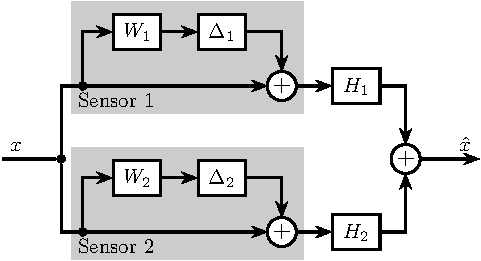
\includegraphics[scale=1]{figs/fusion_gain_mismatch_bis.pdf}
\caption{\label{fig:fusion_gain_mismatch_bis}
Sensor Fusion Architecture with Sensor Dynamical Uncertainty}
\end{figure}

The super sensor dynamics \eqref{eq:super_sensor_dyn_uncertainty} is not longer equal to \(1\) and now depends on the sensor dynamic uncertainties \(W_i(s)\) as well as on the complementary filters \(H_i(s)\).
\begin{equation}
\label{eq:super_sensor_dyn_uncertainty}
  \frac{\hat{x}}{x} = 1 + W_1(s) H_1(s) \Delta_1(s) + W_2(s) H_2(s) \Delta_2(s)
\end{equation}

In order to limit the phase and gain uncertainty of the super sensor, one may want to design the complementary filters to such that \eqref{eq:max_uncertainty_super_sensor} is satisfied.
\begin{equation}
\label{eq:max_uncertainty_super_sensor}
  \begin{aligned}
    & \left|W_1 H_1 \Delta_1\right| + \left|W_2 H_2 \Delta_2\right| \le \epsilon \quad \forall\omega,\ \forall \Delta_i\\
    \Leftrightarrow & \left|W_1 H_1\right| + \left|W_2 H_2\right| \le \epsilon \quad \forall\omega
  \end{aligned}
\end{equation}

Condition \eqref{eq:max_uncertainty_super_sensor} is equivalent as to bound the uncertainty set of the super sensor dynamics in the complex plane by a circle centered on \(1\) with a radius equal to \(\epsilon\) (Fig. \ref{fig:uncertainty_gain_phase_variation_bis}).

\begin{figure}[htbp]
\centering
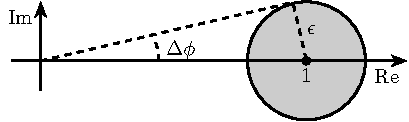
\includegraphics[scale=1]{figs/uncertainty_gain_phase_variation_bis.pdf}
\caption{\label{fig:uncertainty_gain_phase_variation_bis}
Uncertainty set of the super sensor dynamics}
\end{figure}

The maximum phase added by the super sensor uncertainty \(\Delta\phi\) is then equal to \eqref{eq:max_phase_uncertainty}.
\begin{equation}
\label{eq:max_phase_uncertainty}
    \Delta \phi = \arcsin\left( \epsilon \right)
\end{equation}

Limiting the phase added by the super sensor to \(\Delta \phi = \SI{30}{\degree}\) requires that \(H_1(s)\) and \(H_2(s)\) are designed such that \eqref{eq:max_uncertainty_super_sensor} is satisfied with \(\epsilon = \sin(\Delta\phi = \SI{30}{\degree}) = 0.5\).
Thus the norm of the complementary filter \(|H_i|\) for sensor \(i\) should be made small at frequencies where its dynamic uncertainty \(|W_i|\) is large.\par

As stated above, the requirements in terms of noise attenuation and robustness of the sensor fusion architecture can be termed as upper bounds on the norm of the complementary filters.

\section{Complementary Filters Shaping using the \(\mathcal{H}_\infty\) Synthesis}
\label{sec:orgb8fb6f7}
\label{sec:hinf_method}
As shown in Sec. \ref{sec:requirements}, most of the performance requirements for the design of the complementary filters can be expressed as upper bounds on the magnitude of the filters.

Therefore, the \(\mathcal{H}_\infty\) Loop Shaping framework seems adapted for the synthesis of complementary filters.
In this section, a technique for the synthesis complementary filters while specifying uppers bounds on their magnitudes using the \(\mathcal{H}_\infty\) synthesis is presented.
\subsection{Synthesis of Complementary Filters as a \(\mathcal{H}_\infty\) problem}
\label{sec:org3375829}
\label{sec:hinf_synthesis}

The synthesis objective is to shape the norm of two filters \(H_1(s)\) and \(H_2(s)\) while ensuring their complementary property \eqref{eq:comp_filter}.

The synthesis problem is then to find stable transfer functions \(H_1(s)\) and \(H_2(s)\) such that conditions \eqref{eq:comp_filter_problem_form} are satisfied.
\begin{subequations}
\label{eq:comp_filter_problem_form}
  \begin{align}
  & H_1(s) + H_2(s) = 1 \label{eq:hinf_cond_complementarity} \\
  & |H_1(j\omega)| \le \frac{1}{|W_1(j\omega)|} \quad \forall\omega \label{eq:hinf_cond_h1} \\
  & |H_2(j\omega)| \le \frac{1}{|W_2(j\omega)|} \quad \forall\omega \label{eq:hinf_cond_h2}
  \end{align}
\end{subequations}
where \(W_1(s)\) and \(W_2(s)\) are two weighting transfer functions chosen to shape the corresponding filters.

In order to express this synthesis problem into a standard \(\mathcal{H}_\infty\) problem, we use the standard architecture shown on Fig. \ref{fig:h_infinity_robust_fusion} where the generalized plant \(P\) is described by \eqref{eq:generalized_plant}.
\begin{equation}
\label{eq:generalized_plant}
  \begin{bmatrix} z_1 \\ z_2 \\ v \end{bmatrix} = P(s) \begin{bmatrix} w\\u \end{bmatrix}; \quad P(s) = \begin{bmatrix}W_1(s) & -W_1(s) \\ 0 & W_2(s) \\  1 & 0 \end{bmatrix}
\end{equation}

\begin{figure}[htbp]
\centering
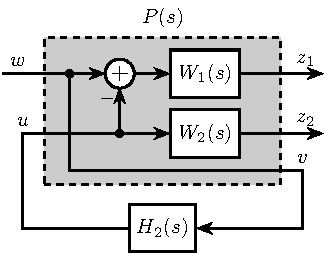
\includegraphics[scale=1]{figs/h_infinity_robust_fusion.pdf}
\caption{\label{fig:h_infinity_robust_fusion}
Architecture used for the \(\mathcal{H}_\infty\) synthesis of complementary filters}
\end{figure}

The \(\mathcal{H}_\infty\) filter design problem is then to find a stable filter \(H_1(s)\) which based on \(v\), generates a signal \(u\) such that the \(\mathcal{H}_\infty\) norm from \(w\) to \([z_1, \ z_2]\) is less than one \eqref{eq:hinf_syn_obj}.
\begin{equation}
\label{eq:hinf_syn_obj}
  \left\|\begin{matrix} \left[1 - H_2(s)\right] W_1(s) \\ H_2(s) W_2(s) \end{matrix}\right\|_\infty \le 1
\end{equation}

Which is equivalent to \eqref{eq:hinf_problem} by defining \(H_1(s) \triangleq 1 - H_2(s)\).
\begin{equation}
\label{eq:hinf_problem}
  \left\|\begin{matrix} H_1(s) W_1(s) \\ H_2(s) W_2(s) \end{matrix}\right\|_\infty \le 1
\end{equation}

The complementary condition \eqref{eq:hinf_cond_complementarity} is ensured by the definition of \(H_1(s)\). The conditions \eqref{eq:hinf_cond_h1} and \eqref{eq:hinf_cond_h2} on the shape of the filters are satisfied by \eqref{eq:hinf_problem}.

Using this \(\mathcal{H}_\infty\) synthesis method, we are then able to shape complementary filters.

\subsection{Choice of the weighting functions}
\label{sec:orgd7d262d}
\label{sec:hinf_weighting_func}

The choice of the weighting functions is of primary importance for the success of the presented \(\mathcal{H}_\infty\) synthesis of complementary filters.

First, only proper, stable and minimum phase transfer functions should be used.
Second, the order of the weights should stay reasonably small as this will increase both the complexity of the optimization problem and the order of the synthesized complementary filters, the latter begin equal to the sum of the weighting functions orders.
Third, one should not forget the fundamental limitations imposed by the complementary property: \(H_1(s) + H_2(s) = 1\).
This implies for instance that \(|H_1(j\omega)|\) and \(|H_2(j\omega)|\) cannot be made small at the same time.


When designing complementary filters, it is usually desired to specify the slope of the filter, its crossover frequency and its low and high frequency gains.
To help with the design of the weighting functions such that the above specification are easily expressed, the formula \eqref{eq:weight_formula} is proposed.
\begin{equation}
\label{eq:weight_formula}
  W(s) = \left( \frac{
           \hfill{} \frac{1}{\omega_0} \sqrt{\frac{1 - \left(\frac{G_0}{G_c}\right)^{\frac{2}{n}}}{1 - \left(\frac{G_c}{G_\infty}\right)^{\frac{2}{n}}}} s + \left(\frac{G_0}{G_c}\right)^{\frac{1}{n}}
         }{
           \left(\frac{1}{G_\infty}\right)^{\frac{1}{n}} \frac{1}{\omega_0} \sqrt{\frac{1 - \left(\frac{G_0}{G_c}\right)^{\frac{2}{n}}}{1 - \left(\frac{G_c}{G_\infty}\right)^{\frac{2}{n}}}} s + \left(\frac{1}{G_c}\right)^{\frac{1}{n}}
         }\right)^n
\end{equation}
where:
\begin{itemize}
\item \(G_0\) is the absolute gain at low frequency
\item \(G_\infty\) is the absolute gain at high frequency
\item \(\omega_0\) and \(G_c\) define the absolute value of the filter at \(\omega = \omega_0\): \(|W(j\omega_0)| = G_c\)
\item \(n\) is the order of the weighting function as well as its slope between high and low frequency
\end{itemize}

The parameters \(G_0\), \(G_c\) and \(G_\infty\) should either satisfy condition \eqref{eq:cond_formula_1} or \eqref{eq:cond_formula_2}.
\begin{subequations}
\label{eq:condition_params_formula}
  \begin{align}
    G_0 < 1 < G_\infty \text{ and } G_0 < G_c < G_\infty \label{eq:cond_formula_1}\\
    G_\infty < 1 < G_0 \text{ and } G_\infty < G_c < G_0 \label{eq:cond_formula_2}
  \end{align}
\end{subequations}

The shape of the weighting function generated using \eqref{eq:weight_formula} is shown on Fig. \ref{fig:weight_formula}.

\begin{figure}[htbp]
\centering
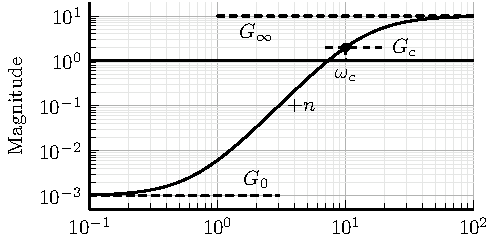
\includegraphics[scale=1]{figs/weight_formula.pdf}
\caption{\label{fig:weight_formula}
Amplitude of the proposed formula for the weighting functions, \(G_0 = 1e^{-3}\), \(G_\infty = 10\), \(\omega_c = \SI{10}{Hz}\), \(G_c = 2\), \(n = 3\)}
\end{figure}

\subsection{Example}
\label{sec:org018b699}
\label{sec:hinf_example}

Let's validate the proposed design method of complementary filters using the \(\mathcal{H}_\infty\) synthesis with a simple example.

Both weighting functions \(W_1(s)\) and \(W_2(s)\) are designed using \eqref{eq:weight_formula}.
The parameters used are summarized on table \ref{tab:weights_params} and the magnitude of the weighting functions are shown on Fig. \ref{fig:hinf_synthesis_results}.

The blending frequency is chosen to be around \(\SI{10}{Hz}\). The slope of \(|H_1(j\omega)|\) is chosen to be \(-2\) above \(\SI{10}{Hz}\) by choosing \(n=2\) for \(W_1(s)\). The slope of \(|H_2(j\omega)|\) is chosen to be \(+3\) below \(\SI{10}{Hz}\) by choosing \(n=3\) for \(W_2(s)\). The order of the obtained complementary filters will thus be of order \(5\).

\begin{table}[htbp]
\caption{\label{tab:weights_params}
Parameters used for \(W_1(s)\) and \(W_2(s)\)}
\centering
\begin{tabularx}{0.5\linewidth}{Xcc}
\toprule
Parameter & \(W_1(s)\) & \(W_2(s)\)\\
\midrule
\(G_0\) & \(0.1\) & \(1000\)\\
\(G_\infty\) & \(1000\) & \(0.1\)\\
\(\omega_c\) [\(\si{Hz}\)] & \(11\) & \(10\)\\
\(G_c\) & \(2\) & \(2\)\\
\(n\) & \(2\) & \(3\)\\
\bottomrule
\end{tabularx}
\end{table}

The bode plot of the obtained complementary filters is shown on Fig. \ref{fig:hinf_synthesis_results} and their transfer functions in the Laplace domain are shown below.
\begin{align*}
  H_1(s) &= \frac{10^{-8} (s+6.6e^9) (s+3450)^2 (s^2 + 49s + 895)}{(s+6.6e^4) (s^2 + 106 s + 3e^3) (s^2 + 72s + 3580)}\\
  H_2(s) &= \frac{(s+6.6e^4) (s+160) (s+4)^3}{(s+6.6e^4) (s^2 + 106 s + 3e^3) (s^2 + 72s + 3580)}
\end{align*}

\begin{figure}[htbp]
\centering
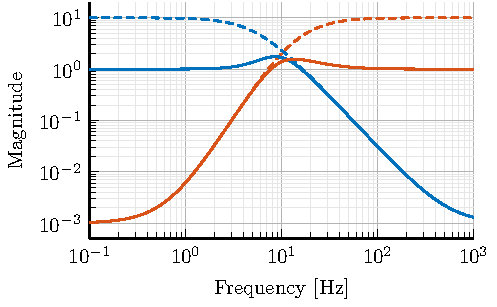
\includegraphics[scale=1]{figs/hinf_synthesis_results.pdf}
\caption{\label{fig:hinf_synthesis_results}
Weighting functions and Obtain Complementary Filters using the \(\mathcal{H}_\infty\) Synthesis}
\end{figure}

\subsection{Generalization to the synthesis of Three Complementary Filters}
\label{sec:orgcb75a24}
\label{sec:hinf_three_comp_filters}
In some applications, it may be needed to merge more than two sensors.
In such case, it is necessary to design as many complementary filters \(H_i(s)\) as the number of sensors used.
The synthesis problem is then to compute \(n\) stable transfer functions \(H_i(s)\) such that \eqref{eq:hinf_problem_gen} is satisfied.
\begin{subequations}
\label{eq:hinf_problem_gen}
  \begin{align}
  & \sum_{i=0}^n H_i(s) = 1 \label{eq:hinf_cond_compl_gen} \\
  & \left| H_i(j\omega) \right| < \frac{1}{\left| W_i(j\omega) \right|}, \quad \forall \omega,\ i = 1 \dots n \label{eq:hinf_cond_perf_gen}
  \end{align}
\end{subequations}
The synthesis architecture on Fig. \ref{fig:h_infinity_robust_fusion} can be generalized for the synthesis of a set of \(n\) complementary filters.
For the synthesis of three complementary filters, the architecture used is shown on Fig. \ref{fig:comp_filter_three_hinf}.

The \(\mathcal{H}_\infty\) synthesis objective applied on \(P(s)\) is to design two stable filters \(H_2(s)\) and \(H_3(s)\) such that the \(\mathcal{H}_\infty\) norm of the transfer function from \(w\) to \([z_1,\ z_2, \ z_3]\) is less than one \eqref{eq:hinf_syn_obj_three}.
\begin{equation}
\label{eq:hinf_syn_obj_three}
  \left\| \begin{matrix} \left[1 - H_2(s) - H_3(s)\right] W_1(s) \\ H_2(s) W_2(s) \\ H_3(s) W_3(s) \end{matrix} \right\|_\infty \le 1
\end{equation}

\begin{figure}[htbp]
\centering
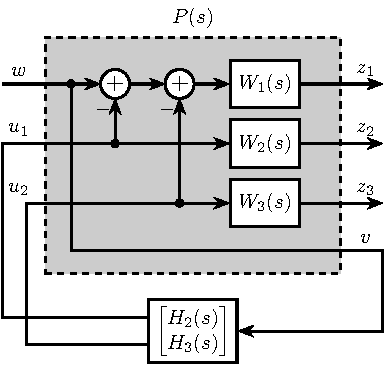
\includegraphics[scale=1]{figs/comp_filter_three_hinf.pdf}
\caption{\label{fig:comp_filter_three_hinf}
Architecture for the \(\mathcal{H}_\infty\) synthesis of three complementary filters}
\end{figure}

By choosing \(H_1(s) \triangleq 1 - H_2(s) - H_3(s)\), the proposed \(\mathcal{H}_\infty\) synthesis solves the design problem \eqref{eq:hinf_problem_gen}. \par
An example is given to validate the method where three sensors are used in different frequency bands (up to \(\SI{1}{Hz}\), from \(1\) to \(\SI{10}{Hz}\) and above \(\SI{10}{Hz}\) respectively).
Three weighting functions are designed using \eqref{eq:weight_formula} and shown by dashed curves on Fig. \ref{fig:hinf_three_synthesis_results}.
The obtained complementary filters after synthesis are shown on Fig. \ref{fig:hinf_three_synthesis_results}.

\begin{figure}[htbp]
\centering
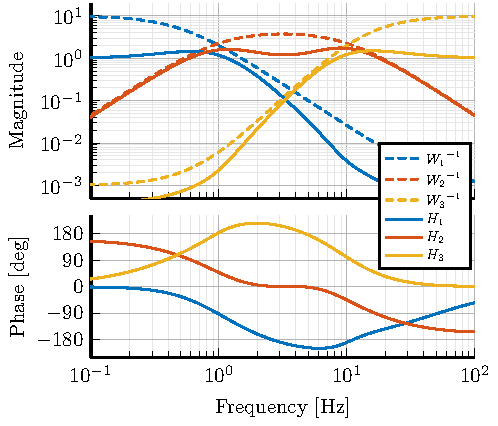
\includegraphics[scale=1]{figs/hinf_three_synthesis_results.pdf}
\caption{\label{fig:hinf_three_synthesis_results}
Obtained three complementary filters}
\end{figure}

\section{Application: Design of Complementary Filters used for the Active Vibration Isolation System at the LIGO}
\label{sec:org8dbdcd2}
\label{sec:application_ligo}
Several complementary filters are used for the active isolation system at the LIGO \cite{hua05_low_ligo,hua04_polyp_fir_compl_filter_contr_system}.
The requirements on those filters are very tight and thus their design is complex.
The approach taken in \cite{hua05_low_ligo} for the design of those filters is to use high order FIR filters and write the synthesis objective as a convex optimization problem.
The obtained FIR filters are compliant with the requirements, however their implementation is complex as it requires a lot of computation power.

In order to demonstrate the effectiveness of the synthesis method presented in section \ref{sec:hinf_method}, complementary filters subject to the same requirements are synthesize.
\subsection{Specifications}
\label{sec:org684e797}
\label{sec:ligo_specifications}

As explained in section \ref{sec:requirements}, typical specifications for the complementary filters are on their magnitude.

The specifications are summarized below and explained in details in \cite{hua04_polyp_fir_compl_filter_contr_system}:
\begin{itemize}
\item From \(0\) to \(\SI{0.008}{Hz}\), the magnitude of the filter's transfer function should be less or equal to \(8 \times 10^{-4}\)
\item Between \(\SI{0.008}{Hz}\) to \(\SI{0.04}{Hz}\), the filter should attenuate the input signal proportional to frequency cubed
\item Between \(\SI{0.04}{Hz}\) to \(\SI{0.1}{Hz}\), the magnitude of the transfer function should be less than \(3\)
\item Above \(\SI{0.1}{Hz}\), the magnitude of the complementary filter should be less than \(0.045\)
\end{itemize}

The specifications are represented by the dashed black curves on the bode plot in Fig. \ref{fig:ligo_weights}.

\subsection{Weighting functions design}
\label{sec:orgac7c8d0}
\label{sec:ligo_weights}
The weighting functions should be designed so that their inverse amplitude is as close as possible to the specifications in order to not over-constrain the synthesis problem.
However, their order should not be too high as to limit both the complexity of the optimization problem and the order of the synthesize complementary filters.

For the weight function corresponding to the low pass filter \(w_L(s)\), a Type I Chebyshev filter of order \(20\) is used. For the one corresponding to the high pass filter \(w_H(s)\), a \(7^{\text{th}}\) order transfer function gives satisfactory results.
The magnitudes of the inverse of the weighting functions are shown on Fig. \ref{fig:ligo_weights}.

\begin{figure}[htbp]
\centering
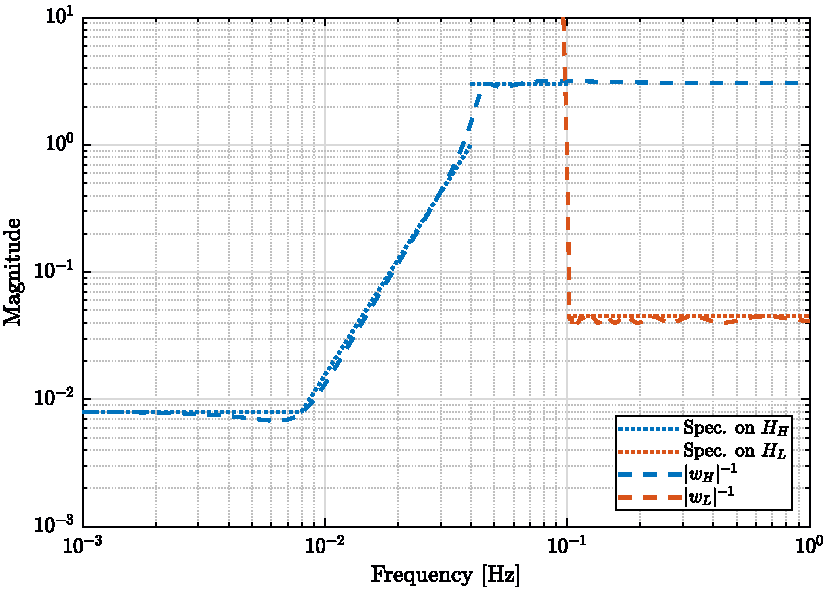
\includegraphics[scale=1]{figs/ligo_weights.pdf}
\caption{\label{fig:ligo_weights}
Specification and Weighting Functions used for the \(\mathcal{H}_\infty\) synthesis}
\end{figure}

\subsection{\(\mathcal{H}_\infty\) Synthesis}
\label{sec:org9dfd8e0}
\label{sec:ligo_results}

The \(\mathcal{H}_\infty\) synthesis is performed using the architecture of Fig. \ref{eq:generalized_plant}.
The complementary filters obtained are of order \(27\).
Their bode plot is compared on Fig. \ref{fig:comp_fir_ligo_hinf} with the FIR filters of order 512 obtained in \cite{hua05_low_ligo}.

\begin{figure}[htbp]
\centering
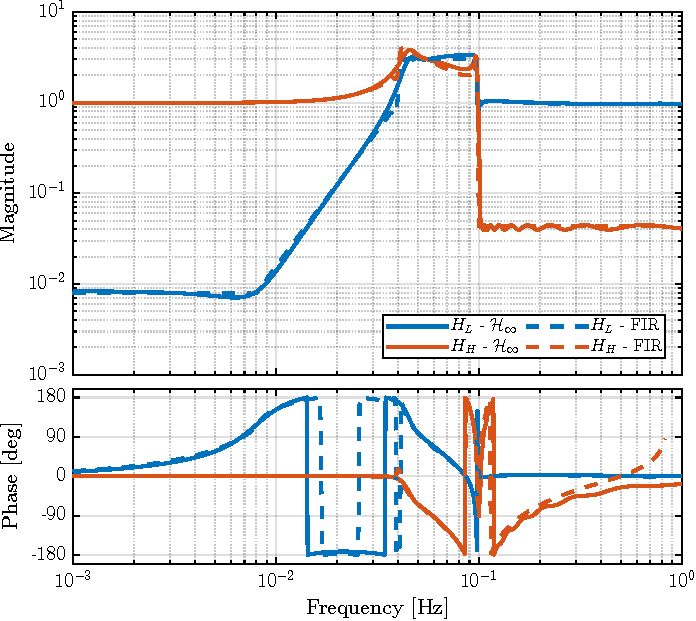
\includegraphics[scale=1]{figs/comp_fir_ligo_hinf.pdf}
\caption{\label{fig:comp_fir_ligo_hinf}
Comparison of the FIR filters (solid) designed in \cite{hua05_low_ligo} with the filters obtained with the \(\mathcal{H}_\infty\) synthesis (dashed)}
\end{figure}

\section{Conclusion}
\label{sec:org30078db}
\label{sec:conclusion}

\section{Acknowledgment}
\label{sec:orgf4d440c}
This research benefited from a FRIA grant from the French Community of Belgium.

\bibliography{ref}
\end{document}